% Editable correction layer over the original V7 vector PDF.
\documentclass[border=0pt]{standalone}
\usepackage[fontset=fandol]{ctex}
\usepackage{graphicx,tikz}
\begin{document}
\begin{tikzpicture}[x=1pt,y=-1pt]
\node[anchor=north west,inner sep=0pt] at (0,0)
  {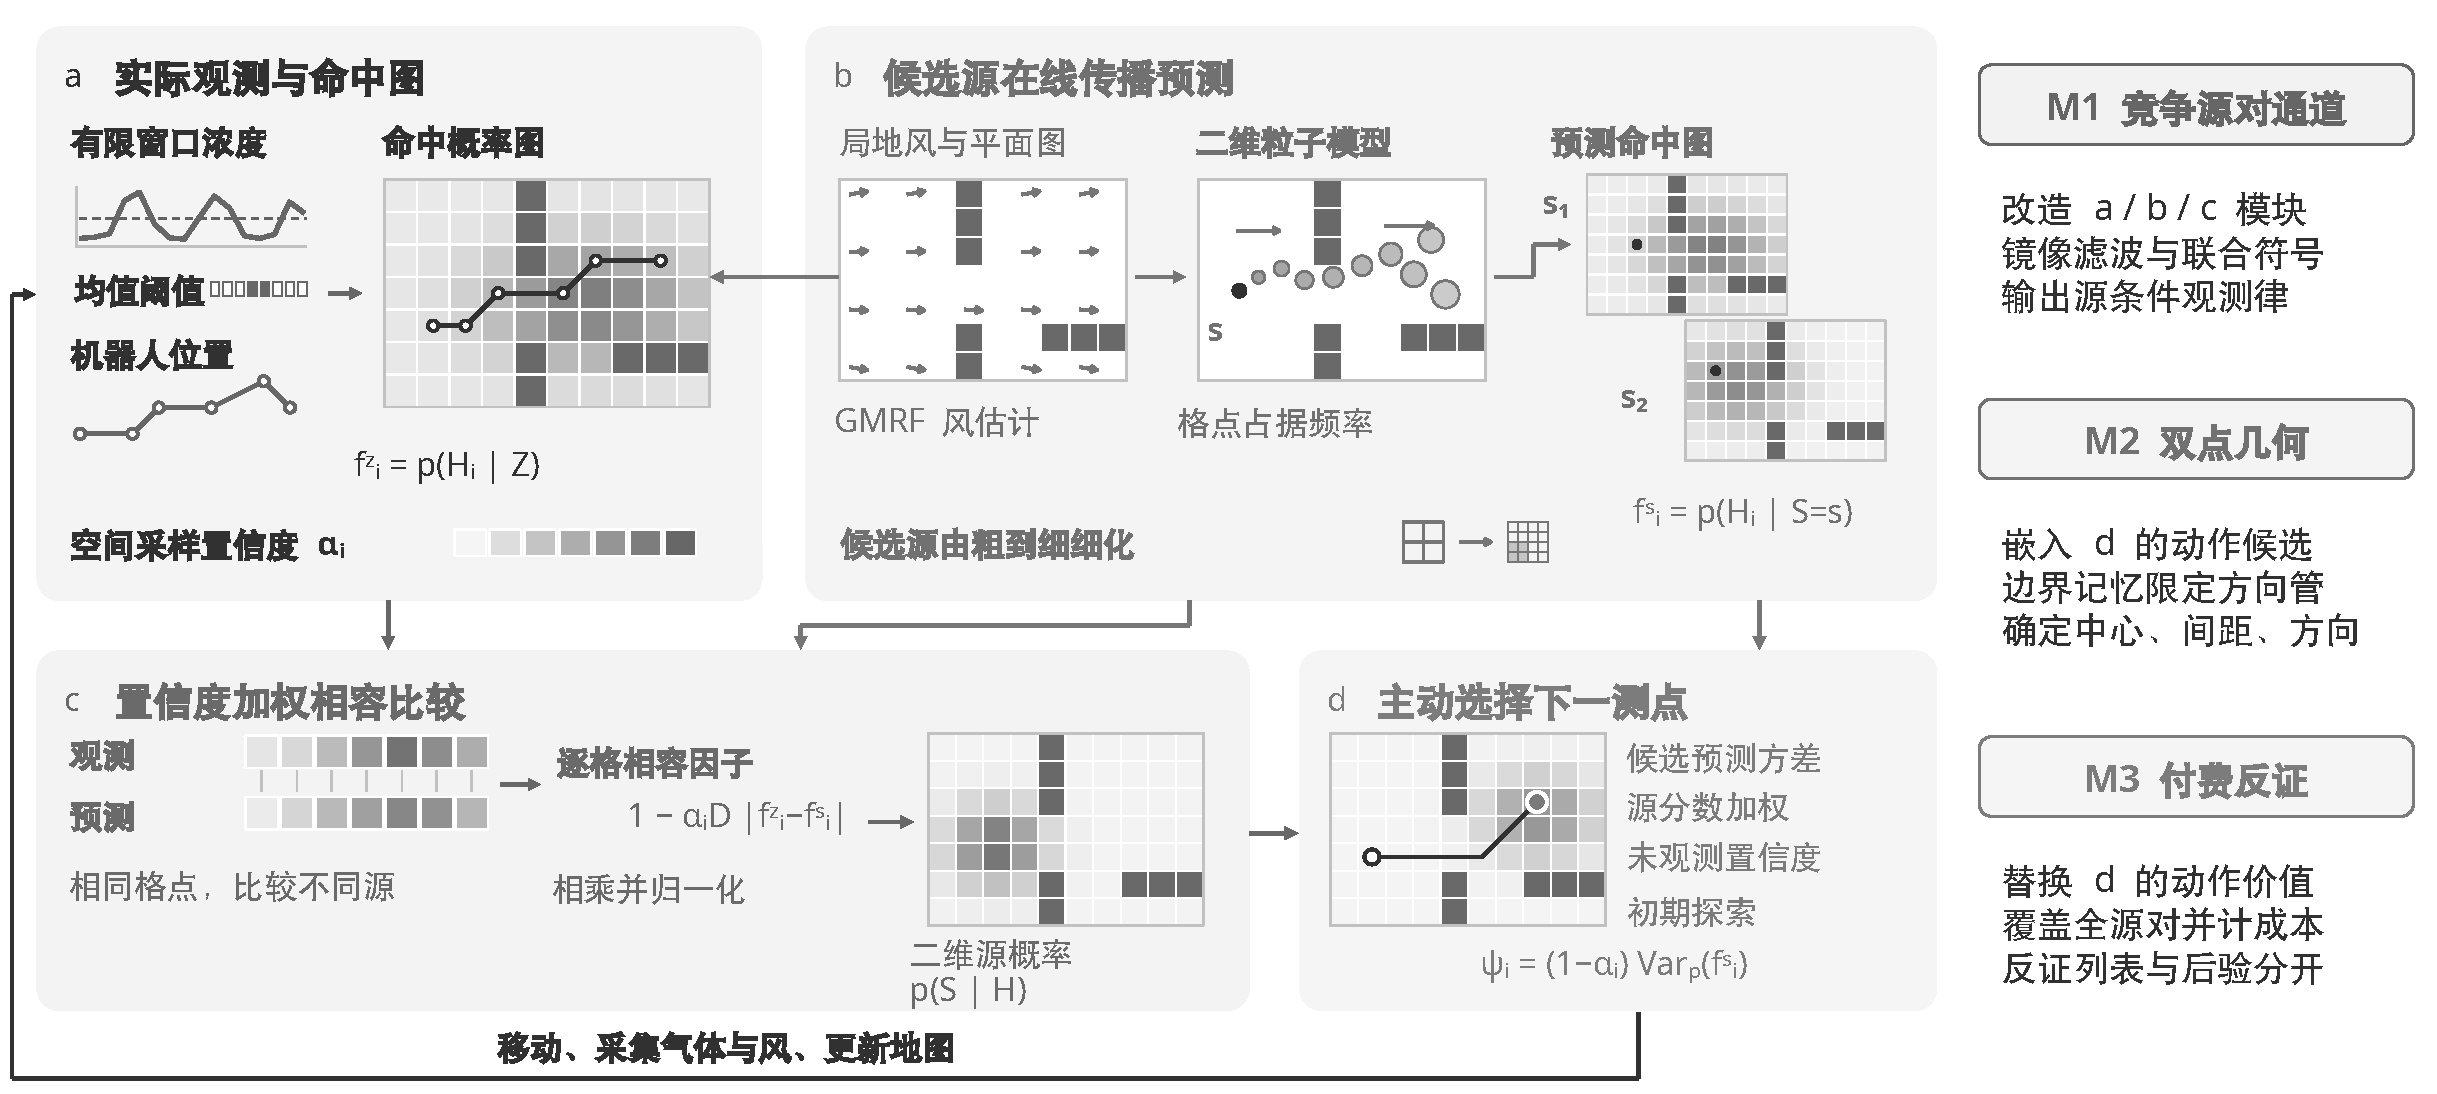
\includegraphics{../figures/fig2_pmfs_original.pdf}};
\fill[black!5] (34,123) rectangle (150,151);
\node[anchor=west,inner sep=0pt,font=\fontsize{16}{18}\selectfont] at (36,137) {均值\,$\to$\,命中};
\fill[white] (951,414) rectangle (1155,476);
\node[anchor=north west,align=left,inner sep=0pt,font=\fontsize{17}{20}\selectfont]
 at (959,414) {完整候选与实际成本\\主假设对全部竞争源\\审计列表与后验分开};
\end{tikzpicture}
\end{document}
